
\حصہء{سوالات}
\موٹا{حصول جذر}\\
\ابتدا{سوال}
\عددی{x_0=-1} لیتے ہوئے ترکیب نیوٹن سے مساوات \عددی{x^2+x-1=0} کا حل حاصل کریں۔  اب \عددی{x_0=1} لیتے ہوئے دوسرا حل تلاش کریں۔دونوں صورتوں میں \عددی{x_2} تلاش کریں۔\\
جواب:\quad
$x_2=\tfrac{13}{21},\, -\tfrac{4}{3}$
\انتہا{سوال}
%==================
\ابتدا{سوال}
\عددی{x_0=0} لیتے ہوئے \عددی{x^3+3x+1=0} کا ایک حقیقی حل ترکیب نیوٹن سے تلاش کریں۔ اس کے بعد \عددی{x_2} تلاش کریں۔
\انتہا{سوال}
%=================
\ابتدا{سوال}
\عددی{x_0=-1} لیتے ہوئے ترکیب نیوٹن سے  تفاعل \عددی{f(x)=x^4+x-3} کا بایاں صفر اور \عددی{x_0=1} لیتے ہوئے اس کا دایاں صفر تلاش کریں۔دونوں صورتوں میں \عددی{x_2} تلاش کریں۔\\
جواب:\quad
$x_2=\tfrac{5763}{4945},\, -\tfrac{51}{31}$
\انتہا{سوال}
%===================
\ابتدا{سوال}
تفاعل \عددی{f(x)=2x-x^2+1} کے دونوں جذر ترکیب نیوٹن سے تلاش کریں۔ \عددی{x_0=0} سے شروع کرتے ہوئے بائیں ہاتھ صفر اور \عددی{x_0=2}سے شروع  کرتے ہوئے دائیں ہاتھ صفر حاصل کریں۔ دونوں صورتوں میں \عددی{x_2} تلاش کریں۔
\انتہا{سوال}
%====================
\ابتدا{سوال}
مساوات \عددی{x^4-2=0} کو حل ترکیب نیوٹن سے  کرتے ہوئے \عددی{2} کا مثبت چوتھا جذر تلاش کریں۔ ابتدائی نقطہ \عددی{x_0=1} لیں۔\عددی{x_2} کیا ہو گا؟\\
جواب:\quad
$x_2=\tfrac{2387}{2000}$
\انتہا{سوال}
%=====================
\ابتدا{سوال}
مساوات \عددی{x^4-2=0} کو حل کرتے ہوئے \عددی{2} کا منفی چوتھا جذر ترکیب نیوٹن سے  تلاش کریں۔ ابتدائی نقطہ \عددی{x_0=-1} لیں۔\عددی{x_2} کیا ہو گا؟
\انتہا{سوال}
%=====================
\ابتدا{سوال}
\عددی{x} کی کس قیمت پر \عددی{\cos x=2x} ہو گا؟ کیلکولیٹر استعمال کریں۔\\
جواب:\quad
$x\approx 0.45$
\انتہا{سوال}
%====================
\ابتدا{سوال}
\عددی{x} کی کس قیمت پر \عددی{\cos x=-x} ہو گا؟ کیلکولیٹر استعمال کریں۔
\انتہا{سوال}
%====================
\ابتدا{سوال}
متوسط قیمت مسئلہ (صفحہ \حوالہصفحہ{مسئلہ_حد_متوسط_قیمت}) استعمال کرتے ہوئے دکھائیں کہ \عددی{f(x)=x^3+2x-4} کا ایک جذر \عددی{x=1} اور \عددی{x=2} کے بیچ پایا جاتا ہے۔ اس جذر کو ترکیب نیوٹن کی مدد سے \عددی{5} اعشاریہ درستگی تک تلاش کریں۔\\
جواب:\quad
$1.17951$
\انتہا{سوال}
%=======================
\ابتدا{سوال}
\عددی{\pi} کی قیمت کا تخمینہ مساوات \عددی{\tan x=0} کے حل سے حاصل کیا جا سکتا ہے۔نقطہ \عددی{x_0=3} سے شروع کرتے ہوئے ترکیب نیوٹن  سے، کیلکولیٹر کی استعمال کے ساتھ،  \عددی{\pi} کی قیمت جتنے اعشاریہ درستگی تک ممکن ہو حاصل کریں۔ 
\انتہا{سوال}
%===================
\موٹا{نظریہ، مثالیں اور استعمال}\\
\ابتدا{سوال}
فرض کریں آپ کا منتخب کردہ ابتدائی نقطہ مساوات \عددی{f(x)=0} کا حل ہوتا ہے۔مزید فرض کریں کہ \عددی{f'(x_0)} معین اور غیر صفر ہے۔ ایسی صورت میں \عددی{x_1} اور دیگر تخمین کیا حاصل ہوں گے؟ 
\انتہا{سوال}
%=======================
\ابتدا{سوال}
آپ \عددی{\tfrac{\pi}{2}} کی قیمت \عددی{5} اعشاریہ درست ترکیب نیوٹن سے \عددی{\cos x=0} حل کرتے ہوئے حاصل کرنا چاہتے ہیں۔ کیا ابتدائی نقطہ کی کوئی اہمیت ہو گی؟ اپنے جواب کی وجہ پیش کریں۔
\انتہا{سوال}
%=====================
\ابتدا{سوال}\شناخت{سوال_استعمال_ارتعاش}\ترچھا{ارتعاش۔}\quad
اگر \عددی{h>0} ہو تب ترکیب نیوٹن استعمال کرتے ہوئے دکھائیں کہ \عددی{x_0=h} منتخب کرتے ہوئے درج ذیل تفاعل کے لئے \عددی{x_1=-h} حاصل ہو گا
\begin{align*}
f(x)=
\begin{cases}
\sqrt{x},&x\ge 0\\
\sqrt{-x},&x<0
\end{cases}
\end{align*}
اور \عددی{x_0=-h} منتخب کرنے سے \عددی{x_1=h} حاصل ہو گا۔اس مسئلے کی ترسیم کھینچ کر اس عمل کی وضاحت کریں۔\\
جواب:\quad شکل \حوالہ{شکل_سوال_استعمال_ارتعاش}
\انتہا{سوال}
%======================
\begin{figure}
\centering
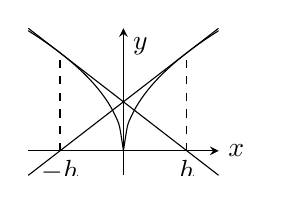
\begin{tikzpicture}[declare function={f(\x)=sqrt(\x);g(\x)=sqrt(-\x);m(\x)=1/(2*sqrt(\x));gm(\x)=-1/(2*sqrt(-\x));}]
\pgfmathsetmacro{\xa}{2}
\pgfmathsetmacro{\yL}{g(-\xa)}
\pgfmathsetmacro{\yR}{f(\xa)}
\begin{axis}[width=4cm,axis lines=middle,xlabel={$x$},ylabel={$y$},xlabel style={at={(current axis.right of origin)},anchor=west},xtick={\empty},ytick={\empty}]
\addplot[domain=0:3,smooth]{f(x)};
\addplot[domain=0:-3,smooth]{g(x)};
\addplot[domain=-3:3]{f(\xa)+m(\xa)*(x-\xa)};
\addplot[domain=-3:3]{g(-\xa)+gm(-\xa)*(x+\xa)};
\draw[dashed](axis cs:-\xa,0)node[below]{$-h$}--(axis cs:-\xa,\yL);
\draw[dashed](axis cs:\xa,0)node[below]{$h$}--(axis cs:\xa,\yR);
\end{axis}
\end{tikzpicture}
\caption{}
\label{شکل_سوال_استعمال_ارتعاش}
\end{figure}
\ابتدا{سوال}\ترچھا{بگڑتی ہوئی تخمین}\quad
تفاعل \عددی{f(x)=x^{\tfrac{1}{3}}} کو ترکیب نیوٹن سے حل کریں۔ ابتدائی نقطہ \عددی{x_0=1} لیتے ہوئے \عددی{x_1}، \عددی{x_2}، \عددی{x_3} اور \عددی{x_4} تلاش کریں۔ \عددی{\abs{x_n}} کا کلیہ کیا ہو گا؟  \عددی{n\to \infty} کرنے سے \عددی{\abs{x_n}} کو کیا ہو گا؟ تصویر کشی کر کے وضاحت کریں۔
\انتہا{سوال}
%========================
\ابتدا{سوال}
سمجھائیں کہ درج ذیل چار فقرے ایک ہی معلومات پوچھ رہی ہیں۔
\begin{enumerate}[a.]
\item
تفاعل \عددی{f(x)=x^3-3x-1} کا جذر تلاش کریں۔
\item
منحنی \عددی{y=x^3} اور خط \عددی{y=3x+1} کی نقطہ تقاطع کا \عددی{x} محدد تلاش کریں۔ 
\item
منحنی \عددی{y=x^3-3x} جہاں \عددی{y=1}کو قطع کرتی ہے اس نقطے کا \عددی{x} محدد تلاش کریں۔
\item
\عددی{x} کی وہ قیمت تلاش کریں جس پر \عددی{g(x)=\tfrac{1}{4}x^4-\tfrac{3}{2}x^2-x+5} کا تفرق صفر ہو گا۔
\end{enumerate}
جواب:\quad
چاروں فقرے جزو-الف کا جذر تلاش کرنے کو کہتے ہیں۔
\انتہا{سوال}
%=========================
\ابتدا{سوال}
ایک سیارے کا مقام تلاش کرنے کی خاطر  ہمیں \عددی{x=1+0.5\sin x} حل کرنا ہو گا۔ تفاعل \عددی{f(x)=x-1-0.5\sin x} کو ترسیم کرتے ہوئے ایک جذر \عددی{x=1.5} کے قریب حاصل ہوتا ہے۔ اس نقطہ سے شروع کرتے ہوئے بہتر حل \عددی{x_1} تلاش کریں۔( \عددی{5} اعشاریہ درست حل  \عددی{x=1.49870} ہے۔)
\انتہا{سوال}
%=======================
\ابتدا{سوال}

\انتہا{سوال}
%============================
